\documentclass[conference]{IEEEtran}
\IEEEoverridecommandlockouts
% The preceding line is only needed to identify funding in the first footnote. If that is unneeded, please comment it out.
% template source is https://www.ieee.org/conferences/publishing/templates.html
\usepackage{array}
% The array package helps with advanced table formatting. 
\usepackage{caption}
% The caption package is used to adjust caption styles.
\usepackage{cite}
\usepackage{amsmath,amssymb,amsfonts}
\usepackage{algorithmic}
\usepackage{graphicx}
\usepackage{textcomp}
\usepackage{xcolor}
\usepackage{comment}

\def\BibTeX{{\rm B\kern-.05em{\sc i\kern-.025em b}\kern-.08em
    T\kern-.1667em\lower.7ex\hbox{E}\kern-.125emX}}
\begin{document}

\title{The Growing Importance of Systems Engineering in Medical Device Development: A Comprehensive Overview}

\author{\IEEEauthorblockN{1\textsuperscript{st} Dinesh Verma, Ph.D}
\IEEEauthorblockA{\textit{School of Systems and Enterprises} \\
\textit{Stevens Institute of Technology}\\
Hoboken, New Jersey \\
dverma@stevens.edu}
\and
\IEEEauthorblockN{2\textsuperscript{nd} Joseph Green}
\IEEEauthorblockA{\textit{Patient Care Systems} \\
\textit{Medtronic}\\
Minneapolis, Minnesota \\
joseph.green@medtronic.com}
\and
\IEEEauthorblockN{3\textsuperscript{rd} Esteban M. Solorzano Zeledon}
\IEEEauthorblockA{\textit{Electronic Medical Systems} \\
\textit{Boston Scientific}\\
Arden Hills, Minnesota \\
solorze@bsci.com}
}

% Figure out if Chris Unger would like to be a contributor to the paper.

\maketitle

% Abstract section
\begin{abstract}
    The medical device industry is experiencing an unprecedented era of 
    growth and innovation, fueled by rapid technological advancements and 
    the escalating complexity of healthcare needs. As medical devices evolve 
    into intricate systems integrating hardware, software, and sophisticated 
    user interfaces, the role of systems engineering has become increasingly 
    vital. This paper delves into the multifaceted role of systems 
    engineering in medical device development, elucidating its pivotal 
    contributions to ensuring the safety, efficacy, and regulatory compliance 
    of these life-saving and life-enhancing technologies. It explores the 
    unique challenges faced by systems engineers in this domain, including 
    the imperative for seamless interdisciplinary collaboration, robust 
    risk management strategies, and unwavering adherence to stringent 
    regulatory standards. Furthermore, the paper presents compelling 
    insights gleaned from a survey of seasoned medical device systems 
    engineers, offering a firsthand perspective on the prevailing 
    challenges, indispensable tools, preferred methodologies, and 
    optimal learning formats in this dynamic field. By illuminating the 
    evolving landscape of medical device systems engineering, this paper 
    aspires to enrich the ongoing discourse on best practices and 
    knowledge dissemination, ultimately fostering the development of 
    safer, more effective, and compliant medical devices that cater 
    to the diverse needs of patients and healthcare providers worldwide.
\end{abstract}

\begin{IEEEkeywords}
    medical device development, systems engineering, regulatory compliance,
    healthcare systems, medical devices
\end{IEEEkeywords}

\section{Introduction}
    According to Section 201(h) of the Federal Food, Drug, and Cosmetic Act, 
    a medical device (system) is “any instrument, machine, contrivance, implant, 
    in vitro reagent that’s intended to treat, cure, prevent, mitigate, 
    diagnose disease” (“21 USC 321: Definitions; Generally,” n.d.).

    The medical device industry stands at the forefront of technological 
    innovation, continuously pushing the boundaries of what is possible in 
    healthcare. Advancements in fields such as artificial intelligence, 
    robotics, miniaturization, and wireless connectivity have paved the way 
    for the development of groundbreaking medical devices that diagnose, 
    treat, and monitor a wide array of medical conditions. However, this 
    progress is accompanied by a growing complexity in medical device design 
    and functionality. Modern medical devices are no longer isolated pieces of 
    equipment; they are intricate systems comprising interconnected hardware, 
    sophisticated software algorithms, and user interfaces that must seamlessly 
    interact with healthcare professionals and patients.

    In this landscape of increasing complexity, systems engineering has 
    emerged as an indispensable discipline. Systems engineering offers a 
    structured and holistic approach to managing the entire lifecycle of 
    medical device development, from the initial conceptualization and design 
    stages to manufacturing, testing, deployment, and post-market surveillance. 
    It provides a framework for ensuring that all components of a medical 
    device work together harmoniously to achieve the desired clinical outcomes 
    while adhering to stringent safety and regulatory requirements.

    As technology advances and healthcare systems become more intricate, 
    the need for a comprehensive text book on systems engineering for medical 
    devices becomes critical. This text book will serve as a valuable resource for 
    systems engineers, healthcare professionals, regulatory experts, and 
    students, ensuring the continued development of safe and effective medical 
    technologies.

\section{The Multifaceted Role of Systems Engineering in Medical Device Development}

    Systems engineering encompasses a wide range of activities and 
    responsibilities throughout the medical device development 
    lifecycle. Its multifaceted role can be summarized as follows:

    \begin{enumerate}
        \item \textbf{Requirements Elicitation and Management:} Systems 
        engineers engage in extensive collaboration with diverse stakeholders, 
        including clinicians, researchers, regulatory experts, and patients, 
        to elicit and define comprehensive requirements for medical devices. 
        This involves translating clinical needs into clear, measurable, 
        and testable technical specifications. Effective requirements 
        management ensures that the final product aligns with user 
        expectations, regulatory standards, and safety guidelines.
        
        \item \textbf{System Architecture and Design:} Systems engineers are 
        responsible for developing a robust and scalable system architecture 
        that outlines the medical device's components, their interactions, and the 
        overall system behavior. This architectural blueprint serves as the 
        foundation for subsequent design and development activities. It 
        considers factors such as performance, reliability, safety, usability, 
        and manufacturability.

        \item \textbf{Risk Management:} A core tenet of systems engineering 
        is the identification and mitigation of risks throughout the entire 
        product lifecycle. In the context of medical devices, risk management 
        is of paramount importance due to the potential impact on patient 
        safety. Systems engineers employ various risk assessment techniques, 
        such as Failure Modes and Effects Analysis (FMEA) and Fault Tree 
        Analysis (FTA), to identify potential hazards and implement 
        appropriate risk mitigation strategies. %Reference IEC 60812:2018

        \item \textbf{Verification and Validation:} Systems engineers design 
        and execute comprehensive verification and validation plans to 
        ensure that the medical device meets its intended use and complies 
        with all applicable regulatory requirements. Verification involves 
        confirming that the device is built according to specifications, 
        while validation ensures that it performs as intended in its 
        intended use environment. This process includes rigorous testing, 
        analysis, and documentation.

        \item \textbf{Regulatory Compliance:} The medical device industry 
        operates within a stringent regulatory framework to protect patient 
        safety and ensure the quality and effectiveness of medical products. 
        Systems engineers play a crucial role in navigating this complex 
        landscape by ensuring that devices adhere to standards set by 
        regulatory bodies such as the Food and Drug Administration (FDA) 
        in the United States and the European Union Medical Device 
        Regulation (EU MDR) in Europe. This involves meticulous 
        documentation, adherence to quality management systems (QMS), 
        and compliance with design control regulations.

        \item \textbf{Interdisciplinary Collaboration:} Medical device 
        development is inherently interdisciplinary, requiring 
        collaboration among experts from diverse fields such as 
        mechanical engineering, electrical engineering, software 
        engineering, materials science, and clinical medicine. Systems 
        engineers act as facilitators and integrators, fostering 
        effective communication and coordination among these teams. 
        They ensure that all aspects of the medical device, from hardware 
        and software to user interfaces and clinical workflows, are 
        seamlessly integrated.
    \end{enumerate}

\section{Systems Engineering in Medical Device Industry}

\section{Unique Challenges in Medical Device Systems Engineering}

    While systems engineering principles are applicable across various 
    industries, the medical device sector presents unique challenges that 
    demand specialized knowledge and expertise. Some of the most salient 
    challenges include:

    \begin{enumerate}
        \item \textbf{Complexity and Integration:} Modern medical 
        devices are characterized by increasing complexity, often 
        incorporating a wide array of technologies, including sensors, 
        actuators, microprocessors, wireless communication modules, 
        and sophisticated software algorithms. Integrating these diverse 
        components into a cohesive and reliable system poses a significant 
        challenge for systems engineers. They must ensure that all 
        subsystems function harmoniously, that data is accurately 
        collected and processed, and that the device operates safely 
        and effectively in various clinical environments.

        \item \textbf{Stringent Regulatory Requirements:} The medical 
        device industry is subject to stringent regulations and 
        standards aimed at safeguarding patient safety and ensuring 
        the quality and performance of medical products. Systems 
        engineers must possess a deep understanding of these 
        regulations, including FDA regulations in the United States, 
        the EU Medical Device Regulation (MDR), and ISO 13485 quality 
        management system standards. Compliance with these regulations 
        necessitates meticulous documentation, rigorous testing, and 
        adherence to design control processes throughout the device 
        lifecycle.

        \item \textbf{Human Factors Engineering:} Medical devices are 
        ultimately used by healthcare professionals and patients, 
        and their design must prioritize usability, safety, and 
        effectiveness in real-world clinical settings. Systems 
        engineers must incorporate human factors engineering 
        principles into the design process, considering factors such 
        as ergonomics, cognitive workload, and potential user errors. 
        This involves conducting user research, task analysis, 
        and usability testing to ensure that the device's interface 
        and functionality are intuitive and user-friendly.

        \item \textbf{Rapid Technological Advancements:} The medical 
        device industry is characterized by a rapid pace of 
        technological innovation. New technologies, such as artificial 
        intelligence, machine learning, 3D printing, and wearable 
        sensors, are constantly emerging and have the potential to 
        revolutionize healthcare. Systems engineers must stay abreast 
        of these advancements and evaluate their applicability to 
        medical device development. Integrating new technologies 
        while maintaining safety, reliability, and regulatory 
        compliance requires careful consideration and a proactive 
        approach.
    \end{enumerate}

\section{How Medical Device Systems Engineering differ to other industries}

Table.~\ref{tab:industry-comparison-part1} and Table.~\ref{tab:industry-comparison-part2} presents a comparative analysis of systems engineering practices 
across four diverse industries: Medical Device, Aerospace, Automotive, 
and Consumer Electronics. Each industry operates within distinct 
regulatory frameworks, market demands, and stakeholder expectations, 
leading to unique approaches in managing safety, performance, cost, 
complexity, and customization in product development.

    \begin{table*}[t]
        \caption{Comparative Analysis of Systems Engineering Characteristics Across Industries: Medical Device, Aerospace, Automotive, and Consumer Electronics (Part 1)}
        \label{tab:industry-comparison-part1}
        \centering
        \begin{tabular}{|p{2.5cm}|p{3.5cm}|p{3.5cm}|p{3.5cm}|p{3.5cm}|}
        \hline
        \textbf{Feature} & \textbf{Medical Device} & \textbf{Aerospace} & \textbf{Automotive} & \textbf{Consumer Electronics} \\ \hline
        \textbf{Focus} & Safety and regulatory compliance (FDA requirements) & Performance, reliability, and safety for critical applications & Safety, cost-effectiveness, and manufacturability & Cost, functionality, and user experience \\ \hline
        \textbf{Life Cycle} & Highly regulated with strict change control processes & Long development cycles with significant upfront investment & Cyclical development with model year changes & Fast-paced development with shorter product lifecycles \\ \hline
        \textbf{Stakeholders} & Broader range including patients, doctors, and regulatory bodies & Primarily engineers, government agencies, and airline customers & Consumers, dealerships, and regulatory bodies & Consumers, retailers, and internal marketing/design teams \\ \hline
        \end{tabular}
    \end{table*}
    
    \begin{table*}[t]
        \caption{Comparative Analysis of Systems Engineering Characteristics Across Industries: Medical Device, Aerospace, Automotive, and Consumer Electronics (Part 2)}
        \label{tab:industry-comparison-part2}
        \centering
        \begin{tabular}{|p{2.5cm}|p{3.5cm}|p{3.5cm}|p{3.5cm}|p{3.5cm}|}
        \hline
        \textbf{Feature} & \textbf{Medical Device} & \textbf{Aerospace} & \textbf{Automotive} & \textbf{Consumer Electronics} \\ \hline
        \textbf{Risk Management} & Extremely high focus on mitigating risks to patient safety & High focus on mitigating risks of catastrophic failure & Focus on safety while balancing cost and manufacturability & Focus on user safety and product liability \\ \hline
        \textbf{Cost Considerations} & Balancing cost-effectiveness with safety and regulatory requirements & Cost is a major driver, but safety remains paramount & Balancing cost with performance and consumer expectations & Cost is a major driver, with emphasis on economies of scale \\ \hline
        \textbf{Complexity} & Devices can be complex with software, hardware, and user interaction & Highly complex systems with long development timelines and extreme performance demands & Complex systems with a focus on integration and manufacturability & Range from simple to complex, with emphasis on user experience and ease of use \\ \hline
        \textbf{Customization} & Typically low customization allowed for medical devices & Limited customization, with focus on platform development for different variants & Some customization for different markets and customer segments & High degree of customization for specific features and functionalities \\ \hline
        \end{tabular}
    \end{table*}

    Table.~\ref{tab:industry_features_part1} and Table.~\ref{tab:industry_features_part2} provides examples of differences between systems 
    engineering in medical device industry and other 
    industries.
    
    % Insert table here

    \begin{table*}[t]
    \caption{Examples of feature differences across industries (Part 1)}
    \label{tab:industry_features_part1}
    \centering
    \begin{tabular}{|p{2.5cm}|p{6.5cm}|p{6.5cm}|}
    \hline
    \textbf{Feature}         & \textbf{Medical Device Industry}                                                                                                                                                                                                                                                                                                                                                                               & \textbf{Other Industries}                                                                                                                                                                                                                                                                                                                                                                                                                                   \\ \hline
    \textbf{Focus}           & Safety and Regulatory Compliance                                                                                                                                                                                                                                                                                                                                                                               & Performance and Technical Specifications                                                                                                                                                                                                                                                                                                                                                                                                                    \\ \hline
    \textbf{Example}         & A cardiac pacemaker is being developed. Systems engineers focus on volume, power efficiency, and therapy performance to achieve optimal therapy performance and longevity.                                                                                                                                                                                                                                     & An airplane wing is being designed. Systems engineers focus on weight, strength, and aerodynamic efficiency to achieve optimal fuel consumption and flight performance.                                                                                                                                                                                                                                                                                     \\ \hline
    \textbf{Life Cycle}      & Highly Variable Regulation and Change Control Processes                                                                                                                                                                                                                                                                                                                                                        & More Flexible and Iterative Development Cycles                                                                                                                                                                                                                                                                                                                                                                                                              \\ \hline
    \textbf{Example}         & A significant software bug is discovered in a blood glucose monitor after initial release. A software patch is prioritized, developed, verified, validated, and released relatively quickly through a field update. A minor software bug is discovered in a remote monitoring system for blood glucose monitors after initial release.  A software patch can be released quickly through a nightly deployment. & During the development of a new car model, engineers discover a significant issue with the Advanced Driver Assistance Systems (ADAS).  A software patch is prioritized, developed, certified, and released relatively quickly through an over-the-air update. During the development of a new car model, engineers discover a minor issue with the infotainment system. A software patch can be released relatively quickly through an over-the-air update. \\ \hline
    \end{tabular}
    \end{table*}

    \begin{table*}[t]
    \caption{Examples of feature differences across industries (Part 2)}
    \label{tab:industry_features_part2}
    \centering
    \begin{tabular}{|p{2.5cm}|p{6.5cm}|p{6.5cm}|}
    \hline
    \textbf{Feature}         & \textbf{Medical Device Industry}                                                                                                                                                                                                                                                                                                                                                                               & \textbf{Other Industries}                                                                                                                                                                                                                                                                                                                                                                                                                                   \\ \hline
    \textbf{Stakeholders}    & Broader Range Including Patients, Doctors, and Regulatory Bodies                                                                                                                                                                                                                                                                                                                                               & Primarily Engineers and Internal Stakeholders                                                                                                                                                                                                                                                                                                                                                                                                               \\ \hline
    \textbf{Example}         & Systems engineers for a new insulin pump consider not only technical specifications but also user needs (e.g., easy for elderly patients to operate) and feedback from doctors regarding functionality and integration with existing hospital systems.                                                                                                                                                         & While developing a new type of engine, the primary focus for systems engineers might be on meeting internal performance targets set by the company and collaborating with mechanical and electrical engineers on achieving those goals.                                                                                                                                                                                                                     \\ \hline
    \textbf{Risk Management} & Focus on Mitigating Risks to Patient Safety                                                                                                                                                                                                                                                                                                                                                                    & Risk Management is Important, But Tolerances May Be Higher                                                                                                                                                                                                                                                                                                                                                                                                  \\ \hline
    \textbf{Example}         & A potential risk identified during the development of a surgical robot is the possibility of unintended arm movement during delicate procedures. Systems engineers use design for reliability to identify the required tolerance for minimizing the risk, and evaluate the design concepts against the required tolerance using cost-benefit analysis and engineering calculations.                            & When designing a new bridge, there's a risk of structural failure during an earthquake. While safety is crucial, there might be a tolerance for a certain level of risk based on cost-benefit analysis and engineering calculations.                                                                                                                                                                                                                        \\ \hline
    \end{tabular}
    \end{table*}

    The main differences between how systems engineering is 
    performed in the medical device industry versus other 
    industries are as follows:

    \begin{enumerate}
        \item Funding and procurement require MedTech to self-fund or 
        seek financing leading to a market-driven expectation. 
        This leads to several differences in the systems 
        engineering role: the need to understand the stakeholder 
        business, negotiate trade-offs between a large number 
        of (conflicting) external stakeholders, and make 
        trade-offs throughout the program duration based on 
        market fluctuations.

        \item The strong, and growing, overlap between Tech and MedTech 
        industries drive stakeholder expectations that MedTech 
        provides similar user experience and cadence as Tech 
        while maintaining reliability expectations of traditional 
        MedTech. This leads to several differences in the systems 
        engineering role: the need to understand and maintain 
        knowledge of current Tech industry trends, adopt or at 
        least accommodate agile methodologies, plan and execute 
        the delivery of incremental value on short(er) timelines, 
        and accommodate/compensate for the lower reliability 
        of Tech products while integrating more of them into 
        the healthcare environment.

        \item The environments of use (i.e., use conditions) are very 
        harsh and difficult to reduce to first principles. This 
        leads to several differences in the systems engineering 
        role: the need to continually reassess applicability 
        of known use conditions, and identify and develop 
        unique models for each application.

        \item The cadence of release is highly variable and highly 
        sensitive to market conditions. This leads to several 
        differences in the systems engineering role: the need 
        to dynamically negotiate and alter project scope based 
        on competitive analysis and announcements, and 
        continually and simultaneously focus on both increasing 
        capability and reducing cost.

    \end{enumerate}

\section{Survey Insights: A Glimpse into the World of Medical Device Systems Engineers}

%Include the survey results visualizations

    To gain a deeper understanding of the challenges and practices 
    in medical device systems engineering, a survey was conducted 
    among 23 professionals working in this field. The survey 
    garnered responses from a diverse group of systems engineers 
    employed at leading medical device companies and regulatory 
    agencies. The survey results shed light on several key aspects 
    of their work:%cite the web link of the survey results

    \begin{enumerate}

        \item \textbf{Primary Challenges:} Figure.~\ref{fig_challenges} 
        shows that respondents identified systems 
        integration, interdisciplinary collaboration, and ensuring safety 
        and efficacy as the most pressing challenges in their daily work. 
        These findings underscore the need for effective communication, 
        coordination, and risk management strategies in medical device 
        development.

        \begin{figure}[htbp]
            \centerline{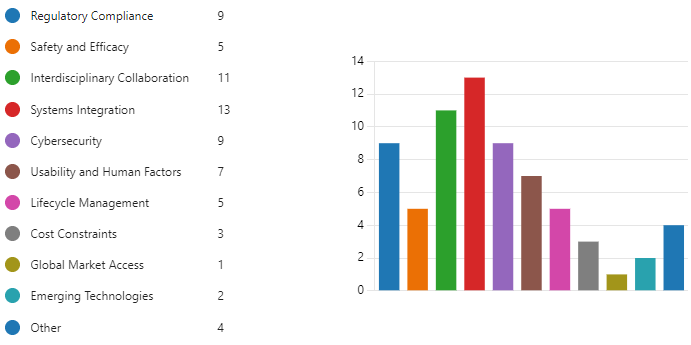
\includegraphics[width=\linewidth]{../report/_book/images/paste-31.png}}
            \caption{Primary challenges encountered in the systems engineering 
            process for medical devices}
            \label{fig_challenges}
        \end{figure}
            
        \item \textbf{Indispensable Tools:} Figure.~\ref{fig_tools} shows that
        requirement management software and documentation tools emerged as the most indispensable tools 
        for medical device systems engineers. This highlights the critical 
        importance of clear, well-defined requirements and meticulous 
        documentation throughout the development process.

        \begin{figure}[htbp]
            \centerline{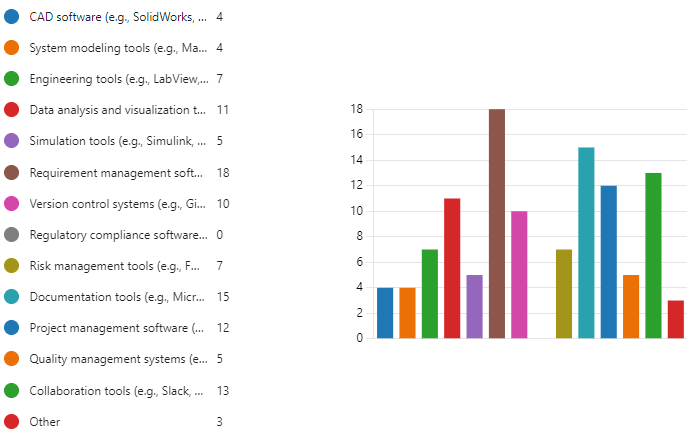
\includegraphics[width=\linewidth]{../report/_book/images/paste-32.png}}
            \caption{Tools indispensable for medical device systems engineer's daily tasks}
            \label{fig_tools}
        \end{figure}
    
        \item \textbf{Beneficial Methodologies:} Figure.~\ref{fig_methods} shows that 
        Model-Based Systems Engineering (MBSE) and quality and compliance methodologies like 
        Failure Modes and Effects Analysis (FMEA) were highly regarded 
        by respondents. These methodologies provide a structured framework 
        for system design, risk assessment, and ensuring regulatory 
        compliance.

        \begin{figure}[htbp]
            \centerline{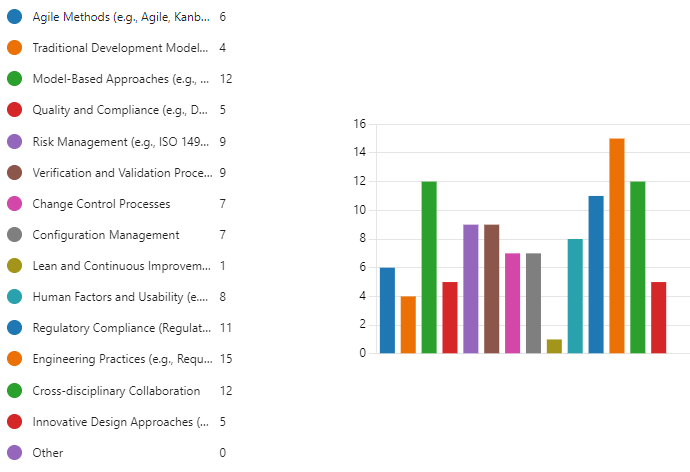
\includegraphics[width=\linewidth]{../report/_book/images/paste-35.png}}
            \caption{Methodologies most beneficial for medical device systems engineer's daily tasks}
            \label{fig_methods}
        \end{figure}
    
        \item \textbf{Learning Preferences:} Figure.~\ref{fig_learning_preferences} shows that the survey revealed a 
        preference for e-books, webinars, and interactive online courses 
        as the most accessible and beneficial learning formats. This suggests 
        a need for educational resources that are readily available, 
        engaging, and tailored to the specific needs of medical device 
        systems engineers.

        \begin{figure}[htbp]
            \centerline{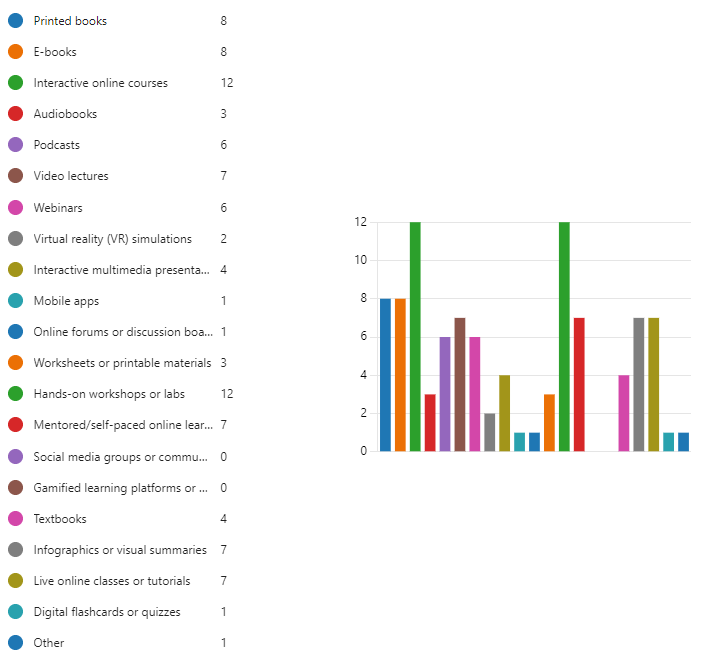
\includegraphics[width=\linewidth]{../report/_book/images/paste-41.png}}
            \caption{Learning formats most accessible and beneficial for medical device systems engineers}
            \label{fig_learning_preferences}
        \end{figure}

    \end{enumerate}

\section{Conclusion}

    In conclusion, systems engineering plays an indispensable role in 
    the development of safe, effective, and compliant medical devices. 
    As the medical device industry continues to evolve at an 
    accelerated pace, systems engineers must rise to the occasion by 
    adapting to new challenges, harnessing emerging technologies, and 
    upholding the highest standards of patient safety. The insights 
    gleaned from this paper and the accompanying survey underscore the 
    importance of continuous education, fostering collaboration across 
    disciplines, and cultivating robust systems engineering practices 
    within the medical device community. By addressing the unique 
    challenges of this field and embracing best practices, systems 
    engineers can make significant contributions to the advancement of 
    medical technology, ultimately improving patient care and outcomes 
    on a global scale.

% Commented content from the IEEE paper template further below.
\begin{comment}
    
\section{Ease of Use}

    \subsection{Maintaining the Integrity of the Specifications}

The IEEEtran class file is used to format your paper and style the text. All margins, 
column widths, line spaces, and text fonts are prescribed; please do not 
alter them. You may note peculiarities. For example, the head margin
measures proportionately more than is customary. This measurement 
and others are deliberate, using specifications that anticipate your paper 
as one part of the entire proceedings, and not as an independent document. 
Please do not revise any of the current designations.



\section{Prepare Your Paper Before Styling}
Before you begin to format your paper, first write and save the content as a 
separate text file. Complete all content and organizational editing before 
formatting. Please note sections \ref{AA}--\ref{SCM} below for more information on 
proofreading, spelling and grammar.

Keep your text and graphic files separate until after the text has been 
formatted and styled. Do not number text heads---{\LaTeX} will do that 
for you.

\subsection{Abbreviations and Acronyms}\label{AA}
Define abbreviations and acronyms the first time they are used in the text, 
even after they have been defined in the abstract. Abbreviations such as 
IEEE, SI, MKS, CGS, ac, dc, and rms do not have to be defined. Do not use 
abbreviations in the title or heads unless they are unavoidable.

\subsection{Units}
\begin{itemize}
\item Use either SI (MKS) or CGS as primary units. (SI units are encouraged.) English units may be used as secondary units (in parentheses). An exception would be the use of English units as identifiers in trade, such as ``3.5-inch disk drive''.
\item Avoid combining SI and CGS units, such as current in amperes and magnetic field in oersteds. This often leads to confusion because equations do not balance dimensionally. If you must use mixed units, clearly state the units for each quantity that you use in an equation.
\item Do not mix complete spellings and abbreviations of units: ``Wb/m\textsuperscript{2}'' or ``webers per square meter'', not ``webers/m\textsuperscript{2}''. Spell out units when they appear in text: ``. . . a few henries'', not ``. . . a few H''.
\item Use a zero before decimal points: ``0.25'', not ``.25''. Use ``cm\textsuperscript{3}'', not ``cc''.)
\end{itemize}

\subsection{Equations}
Number equations consecutively. To make your 
equations more compact, you may use the solidus (~/~), the exp function, or 
appropriate exponents. Italicize Roman symbols for quantities and variables, 
but not Greek symbols. Use a long dash rather than a hyphen for a minus 
sign. Punctuate equations with commas or periods when they are part of a 
sentence, as in:
\begin{equation}
a+b=\gamma\label{eq}
\end{equation}

Be sure that the 
symbols in your equation have been defined before or immediately following 
the equation. Use ``\eqref{eq}'', not ``Eq.~\eqref{eq}'' or ``equation \eqref{eq}'', except at 
the beginning of a sentence: ``Equation \eqref{eq} is . . .''

\subsection{\LaTeX-Specific Advice}

Please use ``soft'' (e.g., \verb|\eqref{Eq}|) cross references instead
of ``hard'' references (e.g., \verb|(1)|). That will make it possible
to combine sections, add equations, or change the order of figures or
citations without having to go through the file line by line.

Please don't use the \verb|{eqnarray}| equation environment. Use
\verb|{align}| or \verb|{IEEEeqnarray}| instead. The \verb|{eqnarray}|
environment leaves unsightly spaces around relation symbols.

Please note that the \verb|{subequations}| environment in {\LaTeX}
will increment the main equation counter even when there are no
equation numbers displayed. If you forget that, you might write an
article in which the equation numbers skip from (17) to (20), causing
the copy editors to wonder if you've discovered a new method of
counting.

{\BibTeX} does not work by magic. It doesn't get the bibliographic
data from thin air but from .bib files. If you use {\BibTeX} to produce a
bibliography you must send the .bib files. 

{\LaTeX} can't read your mind. If you assign the same label to a
subsubsection and a table, you might find that Table I has been cross
referenced as Table IV-B3. 

{\LaTeX} does not have precognitive abilities. If you put a
\verb|\label| command before the command that updates the counter it's
supposed to be using, the label will pick up the last counter to be
cross referenced instead. In particular, a \verb|\label| command
should not go before the caption of a figure or a table.

Do not use \verb|\nonumber| inside the \verb|{array}| environment. It
will not stop equation numbers inside \verb|{array}| (there won't be
any anyway) and it might stop a wanted equation number in the
surrounding equation.

\subsection{Some Common Mistakes}\label{SCM}
\begin{itemize}
\item The word ``data'' is plural, not singular.
\item The subscript for the permeability of vacuum $\mu_{0}$, and other common scientific constants, is zero with subscript formatting, not a lowercase letter ``o''.
\item In American English, commas, semicolons, periods, question and exclamation marks are located within quotation marks only when a complete thought or name is cited, such as a title or full quotation. When quotation marks are used, instead of a bold or italic typeface, to highlight a word or phrase, punctuation should appear outside of the quotation marks. A parenthetical phrase or statement at the end of a sentence is punctuated outside of the closing parenthesis (like this). (A parenthetical sentence is punctuated within the parentheses.)
\item A graph within a graph is an ``inset'', not an ``insert''. The word alternatively is preferred to the word ``alternately'' (unless you really mean something that alternates).
\item Do not use the word ``essentially'' to mean ``approximately'' or ``effectively''.
\item In your paper title, if the words ``that uses'' can accurately replace the word ``using'', capitalize the ``u''; if not, keep using lower-cased.
\item Be aware of the different meanings of the homophones ``affect'' and ``effect'', ``complement'' and ``compliment'', ``discreet'' and ``discrete'', ``principal'' and ``principle''.
\item Do not confuse ``imply'' and ``infer''.
\item The prefix ``non'' is not a word; it should be joined to the word it modifies, usually without a hyphen.
\item There is no period after the ``et'' in the Latin abbreviation ``et al.''.
\item The abbreviation ``i.e.'' means ``that is'', and the abbreviation ``e.g.'' means ``for example''.
\end{itemize}
An excellent style manual for science writers is \cite{b7}.

\subsection{Authors and Affiliations}
\textbf{The class file is designed for, but not limited to, six authors.} A 
minimum of one author is required for all conference articles. Author names 
should be listed starting from left to right and then moving down to the 
next line. This is the author sequence that will be used in future citations 
and by indexing services. Names should not be listed in columns nor group by 
affiliation. Please keep your affiliations as succinct as possible (for 
example, do not differentiate among departments of the same organization).

\subsection{Identify the Headings}
Headings, or heads, are organizational devices that guide the reader through 
your paper. There are two types: component heads and text heads.

Component heads identify the different components of your paper and are not 
topically subordinate to each other. Examples include Acknowledgments and 
References and, for these, the correct style to use is ``Heading 5''. Use 
``figure caption'' for your Figure captions, and ``table head'' for your 
table title. Run-in heads, such as ``Abstract'', will require you to apply a 
style (in this case, italic) in addition to the style provided by the drop 
down menu to differentiate the head from the text.

Text heads organize the topics on a relational, hierarchical basis. For 
example, the paper title is the primary text head because all subsequent 
material relates and elaborates on this one topic. If there are two or more 
sub-topics, the next level head (uppercase Roman numerals) should be used 
and, conversely, if there are not at least two sub-topics, then no subheads 
should be introduced.

\subsection{Figures and Tables}
\paragraph{Positioning Figures and Tables} Place figures and tables at the top and 
bottom of columns. Avoid placing them in the middle of columns. Large 
figures and tables may span across both columns. Figure captions should be 
below the figures; table heads should appear above the tables. Insert 
figures and tables after they are cited in the text. Use the abbreviation 
``Fig.~\ref{fig}'', even at the beginning of a sentence.

\begin{table}[htbp]
\caption{Table Type Styles}
\begin{center}
\begin{tabular}{|c|c|c|c|}
\hline
\textbf{Table}&\multicolumn{3}{|c|}{\textbf{Table Column Head}} \\
\cline{2-4} 
\textbf{Head} & \textbf{\textit{Table column subhead}}& \textbf{\textit{Subhead}}& \textbf{\textit{Subhead}} \\
\hline
copy& More table copy$^{\mathrm{a}}$& &  \\
\hline
\multicolumn{4}{l}{$^{\mathrm{a}}$Sample of a Table footnote.}
\end{tabular}
\label{tab1}
\end{center}
\end{table}

\begin{figure}[htbp]
\centerline{
\includegraphics{fig1.png}}
\caption{Example of a figure caption.}
\label{fig}
\end{figure}

Figure Labels: Use 8 point Times New Roman for Figure labels. Use words 
rather than symbols or abbreviations when writing Figure axis labels to 
avoid confusing the reader. As an example, write the quantity 
``Magnetization'', or ``Magnetization, M'', not just ``M''. If including 
units in the label, present them within parentheses. Do not label axes only 
with units. In the example, write ``Magnetization (A/m)'' or ``Magnetization 
\{A[m(1)]\}'', not just ``A/m''. Do not label axes with a ratio of 
quantities and units. For example, write ``Temperature (K)'', not 
``Temperature/K''.

\section*{Acknowledgment}
\color{red}
The preferred spelling of the word ``acknowledgment'' in America is without 
an ``e'' after the ``g''. Avoid the stilted expression ``one of us (R. B. 
G.) thanks $\ldots$''. Instead, try ``R. B. G. thanks$\ldots$''. Put sponsor 
acknowledgments in the unnumbered footnote on the first page.
\color{black}
\section*{References}

Please number citations consecutively within brackets \cite{b1}. The 
sentence punctuation follows the bracket \cite{b2}. Refer simply to the reference 
number, as in \cite{b3}---do not use ``Ref. \cite{b3}'' or ``reference \cite{b3}'' except at 
the beginning of a sentence: ``Reference \cite{b3} was the first $\ldots$''

Number footnotes separately in superscripts. Place the actual footnote at 
the bottom of the column in which it was cited. Do not put footnotes in the 
abstract or reference list. Use letters for table footnotes.

Unless there are six authors or more give all authors' names; do not use 
``et al.''. Papers that have not been published, even if they have been 
submitted for publication, should be cited as ``unpublished'' \cite{b4}. Papers 
that have been accepted for publication should be cited as ``in press'' \cite{b5}. 
Capitalize only the first word in a paper title, except for proper nouns and 
element symbols.

For papers published in translation journals, please give the English 
citation first, followed by the original foreign-language citation \cite{b6}.


% Need to add the references for the paper
\begin{thebibliography}{00}
\bibitem{b1} G. Eason, B. Noble, and I. N. Sneddon, ``On certain integrals of Lipschitz-Hankel type involving products of Bessel functions,'' Phil. Trans. Roy. Soc. London, vol. A247, pp. 529--551, April 1955.
\bibitem{b2} J. Clerk Maxwell, A Treatise on Electricity and Magnetism, 3rd ed., vol. 2. Oxford: Clarendon, 1892, pp.68--73.
\bibitem{b3} I. S. Jacobs and C. P. Bean, ``Fine particles, thin films and exchange anisotropy,'' in Magnetism, vol. III, G. T. Rado and H. Suhl, Eds. New York: Academic, 1963, pp. 271--350.
\bibitem{b4} K. Elissa, ``Title of paper if known,'' unpublished.
\bibitem{b5} R. Nicole, ``Title of paper with only first word capitalized,'' J. Name Stand. Abbrev., in press.
\bibitem{b6} Y. Yorozu, M. Hirano, K. Oka, and Y. Tagawa, ``Electron spectroscopy studies on magneto-optical media and plastic substrate interface,'' IEEE Transl. J. Magn. Japan, vol. 2, pp. 740--741, August 1987 [Digests 9th Annual Conf. Magnetics Japan, p. 301, 1982].
\bibitem{b7} M. Young, The Technical Writer's Handbook. Mill Valley, CA: University Science, 1989.
\end{thebibliography}

%\vspace{12pt}
%\color{red}
%IEEE conference templates contain guidance text for composing and formatting conference papers. Please ensure that all template text is removed from your conference paper prior to submission to the conference. Failure to remove the template text from your paper may result in your paper not being published.

\end{comment}

\end{document}
